\documentclass{article}
\usepackage{graphicx, enumitem, hyperref}
\usepackage[margin=1in]{geometry}

\title{\textbf{Simdezvous}\\\vspace{0.1in}\large{Rendezvous and docking simulator for\\LEO CubeSats}\vspace{1in}}
\author{Shreeja Shrijan Shrestha\\Rishav Mani Sharma}

\begin{document}

% \setlength{\parindent}{0pt}
\setlength{\parskip}{0.5em}

\maketitle
\newpage

\tableofcontents
\newpage

\section{Feedback}

Atheel asked us to work on demonstrating the disturbance that the electromagnets will cause on the attitude control of a satellite. We don't need to consider two satellites.

\begin{enumerate}[noitemsep]
  \item GUI with following user inputs:
  \begin{enumerate}[noitemsep]
    \item Moment of inertia tensor of a satellite.
    \item Orbital parameters.
    \item Actuator parameters; reaction wheel and magnetorquers.
  \end{enumerate}
  \item Visualize the magnetic field vector of the Earth at a location compared to the orientation of the satellite. Direction of magnetic field of the Earth will be the setpoint of the attitude control such that the electromagnets align with the field.
  \item Perform attitude control and allow the satellite be stable on desired orientation.
  \item Suddenly enable the electromagnets and study their disturbance on the attitude control.
  \item Can theoretical arguments can be made on this scenario?
\end{enumerate}

Atheel suggested the \texttt{CONTROL LAW} in the Figure \ref{fig:architecture} to be composed of three components:

\begin{enumerate}[noitemsep]
  \item Attitude controller with reaction wheel and magnetorquers.
  \item Rendezvous controller with a thruster and attitude controller.
  \item Docking controller with electromagnets (no dependence on the attitude control).
\end{enumerate}

\section{Introduction}

\begin{figure}[ht]
  \centering
  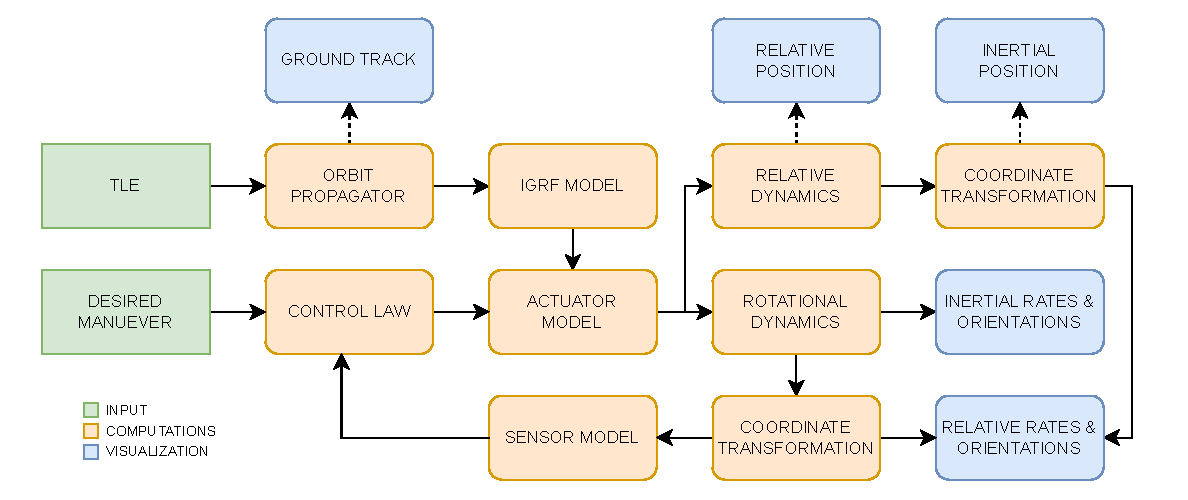
\includegraphics[scale=0.7]{assets/architecture.pdf}
  \caption{Architecture of Simdezvous.}
  \label{fig:architecture}
\end{figure}

Figure \ref{fig:architecture} shows the general architecture of Simdezvous. The orbital information about the satellites are input using TLE (Two Line Elements). TLE is used as initial condition for the orbit propagator which is in turn used to compute the magnetic field using IGRF model. The interaction of magnetic field of the Earth and that of the electromagnets onboard Tamariw can be used to study the affect of Earth's field in the performance of electromagnetic docking of satellites. There are two actuators on Tamariw satellites; a thruster and four electromagnets each. Control commands to actuate these actuators comes from the control law which takes the desired manuever as the set point and the output of sensor model as the feedback of relative position, velocity, orientation, and angular rates. Once actuator delivers forces and torques to the satellite system which affects the relative position and the rotational dynamics of the satellites.

The simulator offers visualization of following parameters:

\begin{enumerate}[noitemsep]
  \item Ground track of the satellites.
  \item Relative position of the satellites in both graph and 3D visualization. The POV can be toggled from one satellite to the other.
  \item Position of the satellites in inertial frame of reference.
  \item Relative orientation and angular rates in 3D visualization. The POV can be toggled from one satellite to the other.
  \item Orientation and angular rates as seen from inertial frame of reference.
\end{enumerate}

\section{Progress}

Following progress has been made so far in the project:

\begin{enumerate}[noitemsep]
  \item Implementation of the Kepler's orbit propagator.
  \item Import and manipulation of the CAD model fo Tamariw satellites in 6DOF and Earth.
  \item Implementation of numerical integration of the Hills differential equations.
\end{enumerate}

We have considered following steps as immediate next steps to the project.

\begin{enumerate}[noitemsep]
  \item Feed the output of the Kepler's orbit propagator to the ground track visualizer.
  \item Visualize the CAD model of Tamariw using the output of Hill equations.
\end{enumerate}

\subsection{Orbit propagator}

Kepler's orbit propagator with J2 effect is implemented and validated with the result published in Curtis' \textit{Orbital Mechanics for Engineering Students}. The validation can be seen by comparing Figure \ref{fig:curtis_ground_track} and Figure \ref{fig:ground_track}. Following parameters are used for both simulations.

\begin{enumerate}[noitemsep]
  \item Perigee = 6700 km
  \item Apogee = 10000 km
  \item Semimajor axis = 8350 km
  \item Eccentricity = 0.197605
  \item Inclination = 1.0472 rad
  \item Periapsis argument = 0.785398 rad
  \item Longitude of ascending node = 4.71239 rad
  \item True anomaly = 4.01426 rad
\end{enumerate}

\begin{figure}[ht]
  \centering
  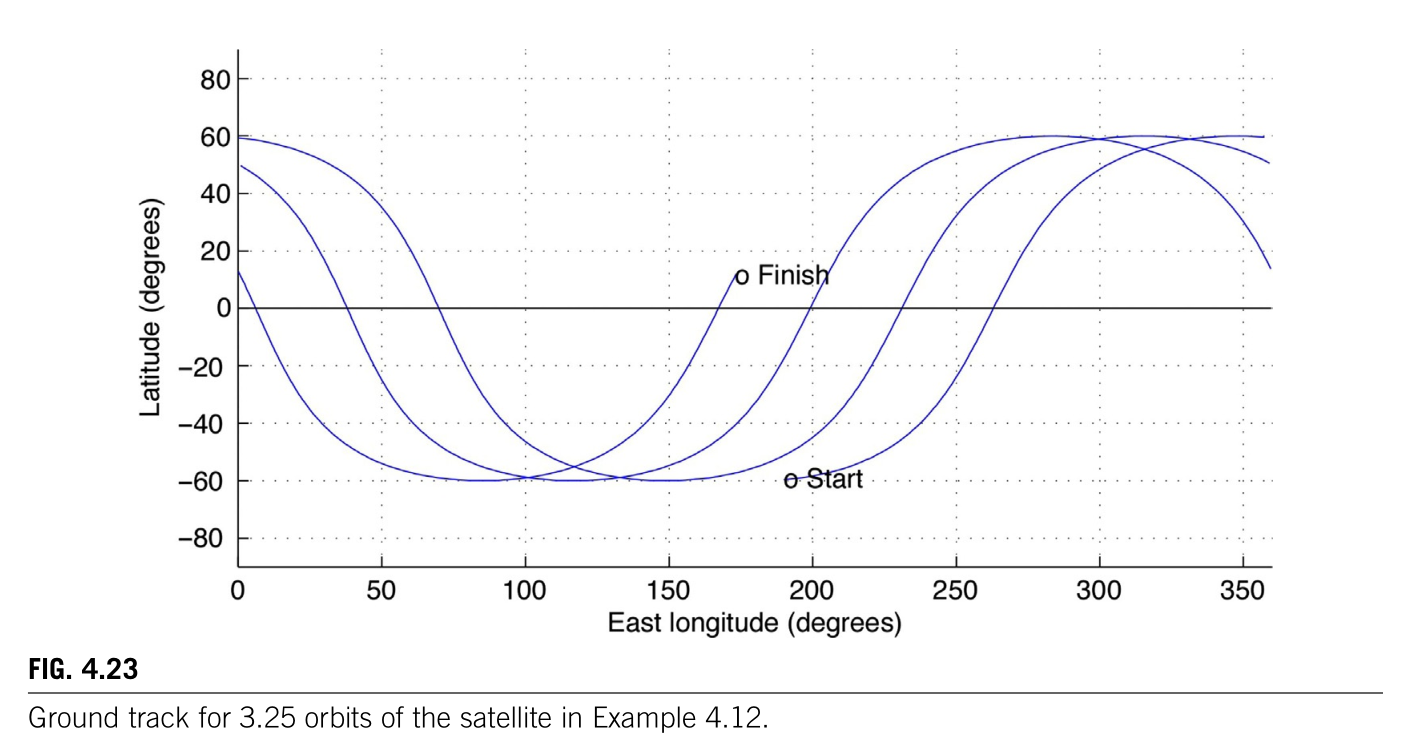
\includegraphics[scale=0.25]{assets/curtis_ground_track.png}
  \caption{Result of Curtis's implementaion of Kepler's orbit propagator.}
  \label{fig:curtis_ground_track}
\end{figure}

\begin{figure}[ht]
  \centering
  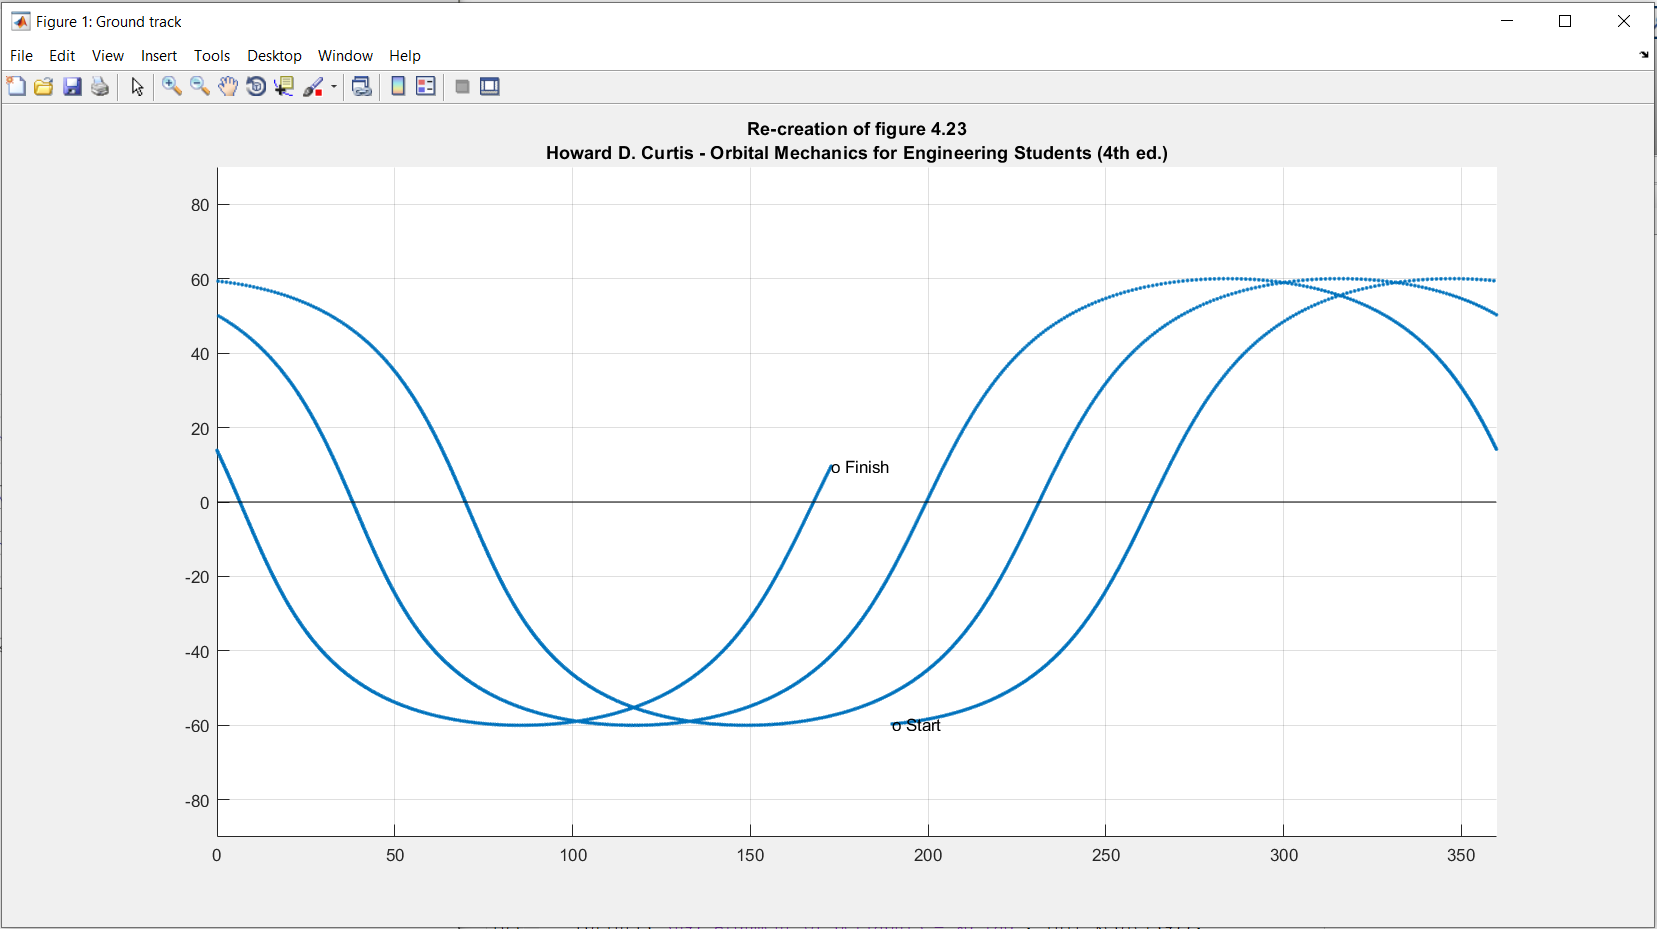
\includegraphics[scale=0.2]{assets/simdezvous_ground_track.png}
  \caption{Our implementation of the ground track using initial condition provided in Curtis' book.}
  \label{fig:ground_track}
\end{figure}

\end{document}
